\chapter{Wybrane fragmenty kodu źródłowego}

\begin{figure}
	\centering
	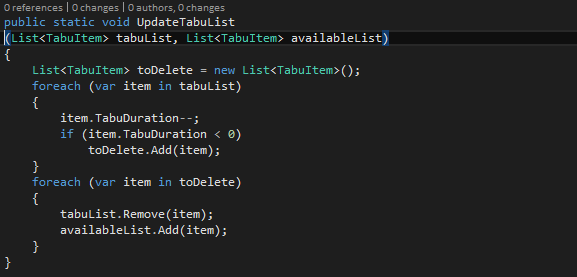
\includegraphics[width=\textwidth] {KOD2}
	\caption{Funkcja aktualizująca listę tabu. }
	\label{fig: KOD2}
\end{figure}

\begin{figure}
	\centering
	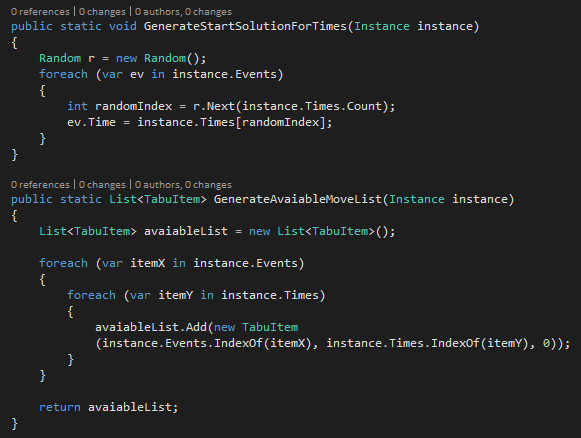
\includegraphics[width=\textwidth] {KOD1}
	\caption{Funkcje generujące rozwiązanie początkowe oraz dostępne ruchy. }
	\label{fig: KOD1}
\end{figure}


\begin{figure}
	\centering
	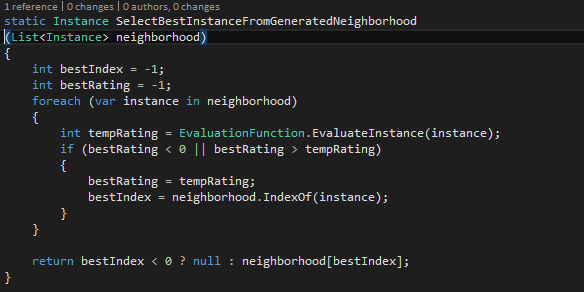
\includegraphics[width=\textwidth] {KOD3}
	\caption{Funkcja wybierająca najlepsze rozwiązanie z sąsiedztwa. }
	\label{fig: KOD3}
\end{figure}

\begin{figure}
	\centering
	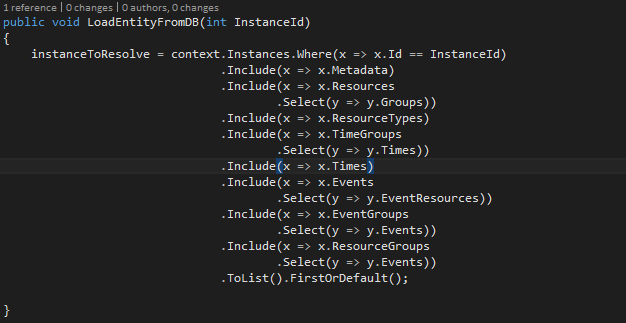
\includegraphics[width=\textwidth] {KOD4}
	\caption{Funkcja wczytująca instancje z bazy danych. }
	\label{fig: KOD4}
\end{figure}

\begin{figure}
	\centering
	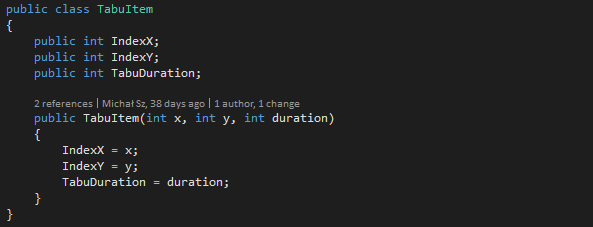
\includegraphics[width=\textwidth] {KOD5}
	\caption{Klasa reprezentująca pojedynczy element na liście tabu. }
	\label{fig: KOD5}
\end{figure}

\begin{figure}
	\centering
	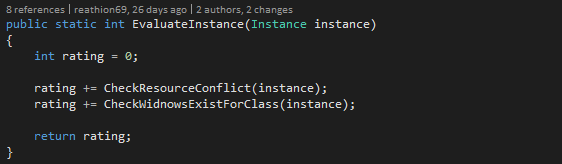
\includegraphics[width=\textwidth] {KOD6}
	\caption{Funkcja oceniająca rozwiązanie. }
	\label{fig: KOD6}
\end{figure}

\begin{figure}
	\centering
	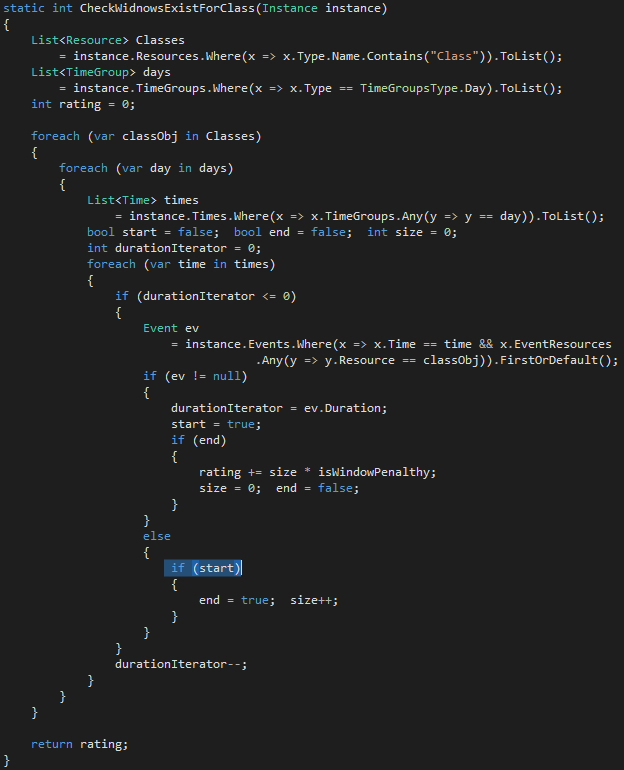
\includegraphics[width=\textwidth] {KOD7}
	\caption{Funkcja sprawdzająca występowanie okienek. }
	\label{fig: KOD7}
\end{figure}

\begin{figure}
	\centering
	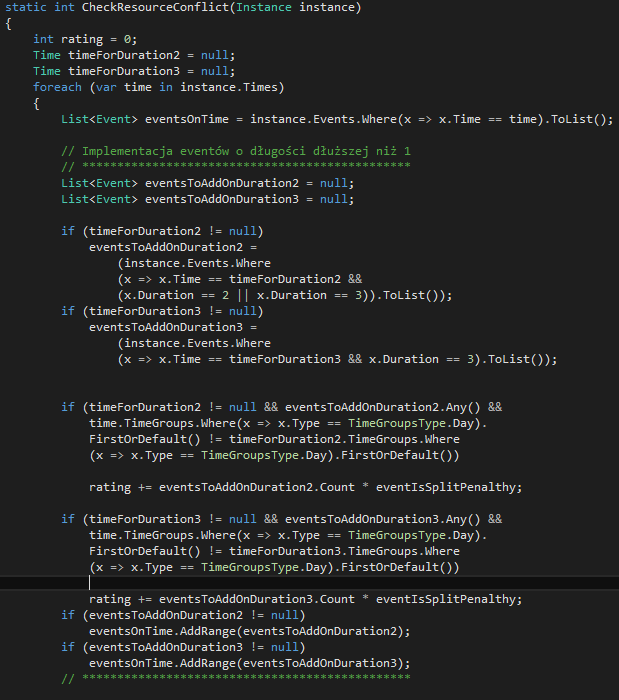
\includegraphics[width=\textwidth] {KOD8}
	\caption{Funkcja sprawdzająca konflikt zasobów oraz ich niepodzielność. Część 1. }
	\label{fig: KOD8}
\end{figure}

\begin{figure}
	\centering
	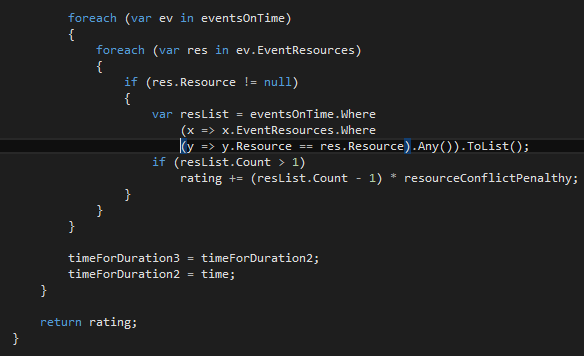
\includegraphics[width=\textwidth] {KOD9}
	\caption{Funkcja sprawdzająca konflikt zasobów oraz ich niepodzielność. Część 2. }
	\label{fig: KOD9}
\end{figure}


%%%%%%%%%%%%%%%%%%%%%%%%%%%%%%%%%%%%%%%%%%%%%%%%%%%%%%%%
